\chapter{Markup}
A manuscript can be a seamless current of words and still make perfect sense to
the author. To truly capture its meaning in a clear and unambiguous manner,
however, the manuscript will often need to be supplemented with a set of
annotations. At a more basic level, this refers to the compliance with the
orthographic rules---such as the correct spelling, capitalization, word breaks,
and punctuation---that are specific to the language of the document.  It is not
at all unreasonable to expect that this basic compliance should be already met
by the manuscript. At a higher level, this consists of discovering and marking
up the inner order and logic of the text, so that the resulting document can
later be typeset in a way that visually reflects its structure.

More often than not, the writing and marking up of a text are two inseparably
connected activities performed in parallel rather than in succession.
Nevertheless, each represents a distinct concept: Writing is the process of
breaking ideas into fragmented strings of words, which the markup reassembles
back into meaningful units of linguistic thought waiting to be brought to life
by a designer.

\index{markup!logical|(}\index{markup!presentation|(}
Markup can be created using a variety of \termpl*{markup language}. Aside from
\term*{logical markup}, which captures the logical structure of a document,
markup languages may also provide \term*{presentation markup}, which directly
impacts the visual properties of the document but carries no semantic
information. The usage of presentation markup makes it impossible to separate
the markup from the design and to capture the logic of the text. As a result,
the consistency in the design of each logical part of the document needs to be
ensured manually, and future changes of design become error-prone and tedious.
In this regard, logical markup is to design what style guides are to writing: a
means of ensuring consistency that should be used whenever possible.
\index{markup!logical|)}\index{markup!presentation|)}

\section{Meta Markup Languages}
\subsection{The General Markup Language}
The situation engulfing digital typesetting was growing increasingly frustrating
for publishers in the 1960s. The markup languages used by different typesetting
systems varied wildly and once a publisher had a large collection of documents
typeset via a given company, switching to another one could be a costly
venture. This power imbalance artificially increased the price of digital
typesetting, leading to a demand for a universal markup language.

This demand was met by a project developed\footnote{
  More information about the project can be found within
  \citework{goldfarb96} and \citework*(SGML: The Reason Why and the First
  Published Hint)[]{goldfarb97:whySGML}.
} at the Cambridge Scientific Center of \acronym{IBM} in the early 1970s. The
project aimed at imbuing a text editor with the ability to query, edit, and
display documents from a repository to allow the usage of computers in legal
practice. Very early on in the development process, it became clear that the
crux was going to be the markup languages in which the documents were written.
These languages were not unified and many of them comprised largely presentation
markup, which made information retrieval impossible without the use of
heuristics. To resolve these issues, a unifying markup language called
\acronym{GML} was drafted. The language was released \cite{goldfarb81}
to the public in \citeyear{goldfarb81} and finally standardized in
\citeyear{iso86} as \acronym{SGML}\footnote{
  The authoritative resource on \acronym{SGML} is \citework{goldfarb91}, which
  includes the full text of the standard bearing extensive annotations.
} \cite{iso86}.

\Acronym{SGML} documents consist of text mixed with \termpl*{tag}%
\acroindex[!tag]{SGML}, which delimit meaningful sections of the document called
\termpl*{element}\acroindex[!element]{SGML}. Elements can carry additional
information in \termpl*{attribute}\acroindex[!attribute]{SGML}. Additionally,
\acronym{SGML} documents may contain miscellaneous instructions for the program
that is processing it, as well as human-readable comments. Repeated strings of
text can be declared as \termpl*[entities]{entity} \acroindex[!entity]{SGML}
that can consequently be used throughout the document in place of the original
strings.

Although the described structure is shared by all \acronym{SGML} documents, the
actual syntax, as well as the restrictions regarding the contents and the
attributes of individual elements, are declared within a \acronym{DTD}, which
can be different for each document. It is worth noting that a \acronym{DTD} only
declares the syntax of an \acroshort{SGML} document; the semantics of the
individual elements and their attributes are left to the interpretation of the
program processing the document. The syntax and the constraints imposed by a
\acronym{DTD} define an \term*{application of \acronym{SGML}}%
\acroindex[!application]{SGML}. An \acronym{SGML} document is considered to be a
valid instance of an \acroshort{SGML} application, when it conforms to the
respective \acronym{DTD}.

\subsection{The Extensible Markup Language}
Although \acronym{SGML} was designed to be the general format for data exchange,
the complexity of the specification and the lack of support for Unicode proved
to be a major hindrance preventing its wider adoption and tool development. In a
response, \acronym{W3C} published a specification of \acronym{XML} in
\citeyear{bray98}. Along with the introduction of \acronym{XML}, the
\acroshort{SGML} specification received a technical corrigendum
\cite{goldfarb97:webSGML}, which turned \acronym{XML} into a proper subset of
\acronym{SGML} restrained by an \acroshort{SGML} \acronym{DTD}.

\begin{figure}
  \inputcode[xml]{examples/02/recipe.xml}
  \caption{An example \acronym{XML} document\filenamecap{recipe.xml}}
  \label{fig:recipe}\bigskip
\end{figure}

\begin{figure}
  \ffootnote{\acronym{SGML} and \acronym{XML} \acronym{DTD}s can be either linked
    to a document through \code[dtd]{PUBLIC} and \code[dtd]{SYSTEM} identifiers,
    directly embedded in a document, linked to a document and then extended by
    an embedded specification, or left out altogether.}
  \inputcode[dtd]{examples/02/dtdtypes}
  \caption{An example recipe \acronym{DTD}}
  \label{fig:recipe-dtd}
\end{figure}
        
\begin{figure}
  \inputcode{examples/02/recipe.rnc}
  \caption{A reformulation of the recipe \acronym{DTD} from Figure
    \ref{fig:recipe-dtd} in the compact syntax of the \acronym{Relax NG}
    schema language\filenamecap{recipe.rnc}}
  \label{fig:recipe-rnc}
\end{figure}

This \acronym{DTD} completely fixes the syntax of \acronym{XML} documents, which
makes it possible to differentiate two levels of correctness. An \acronym{XML}
document is considered to be \term*{well-formed}%
\acroindex[!well-formedness]{XML}, when it conforms to the \acroshort{SGML}
\acronym{DTD} that restrain the syntax of \acronym{XML} as well as to the
specification. An \acroshort{XML} document is considered to be \term*{valid}
\acroindex[!validity]{XML} against an \acroshort{XML} \acronym{DTD}, when it is
well-formed and conforms to the said \acronym{XML} \acronym{DTD}.  Along with
\acronym{DTD}s, there exists a wealth of \termpl*{schema
language}\acroindex[!schema language]{XML}\footnote{
  A list of tools for the manipulation of files in \acronym{XML} schema
  languages is maintained on the Web site of \acronym{W3C} at
  \url{http://www.w3.org/XML/Schema}.
} for \acronym{XML}, such as \acroshort{W3C} \acroshort{XML} Schema%
\acroindex[!Schema]{XML}, \acronym{Relax NG}, or Schematron that can be used to
check the validity of an \acroshort{XML} document instead of a \acronym{DTD}.
The constrains imposed by either a \acronym{DTD} or a schema define an
\term*{application}, \term*{language}, or \term*{format of \acronym{XML}}.
\acroindex[!application]{XML} \acroindex[!language]{XML}
\acroindex[!format]{XML}

\begin{figure}
  \inputcode[xml]{examples/02/recipe.xsd}
  \caption{A reformulation of the recipe \acronym{DTD} from Figure
    \ref{fig:recipe-dtd} in the \acroshort{XML} Schema \acroindex[!Schema]{XML}
    language\filenamecap{recipe.xsd}}
  \label{fig:recipe-xsd}
\end{figure}

\begin{figure}
  \inputcode[sh]{examples/02/recipe.sh}
  \caption{\acronym{XML} documents can be easily validated against \acronym{XML}
    schemata using command-line tools, such as \cliutil{xmllint}.}
\end{figure}

Along with schema languages, other supplementary languages also exist, such as
\inx{XPointer}, \inx{XPath}, and \inx{XQuery} for addressing sets of elements
(fragments) within a \acronym{XML} document or \acronym{CSS} for specifying the
visual properties of an \acroshort{XML} document.

\begin{figure}[!b]
  {\tikzstyle{level 1}=[sibling distance=\baselineskip, level distance=1.5cm]
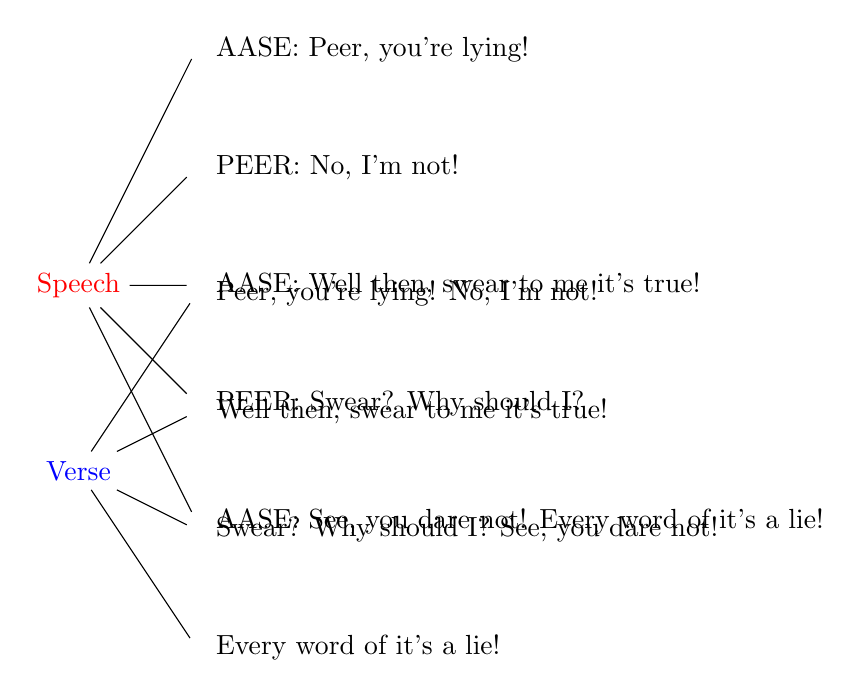
\begin{tikzpicture}[grow=right]
  \node {\textcolor{red}{Speech}}
    child {
      node [label=right:{AASE: See, you dare not! Every word of it's a
        lie!} ] {}}
    child {
      node[label=right:{PEER: Swear? Why should I?}] {} }
    child {
      node[label=right:{AASE: Well then, swear to me it's true!}] {}}
    child {
      node[label=right:{PEER: No, I'm not!}] {} }
    child {
      node[label=right:{AASE: Peer, you're lying!}] {} };
  \node [below=5\baselineskip] {\textcolor{blue}{Verse}}
    child {
      node[label=right:{Every word of it's a lie!} ] {}}
    child {
      node[label=right:{Swear? Why should I? See, you dare not!}] {} }
    child {
      node[label=right:{Well then, swear to me it's true!}] {}}
    child {
      node[label=right:{Peer, you're lying! No, I'm not!}] {} };
\end{tikzpicture}}%
\begin{Verbatim}[commandchars=\\\{\},codes={\catcode`$=3\catcode`^=7\catcode`_=8}]
<(\textcolor{blue}{V})line>
  <(\textcolor{red}{S})speech who="Aase">Peer, you're lying!</(\textcolor{red}{S})speech>
  <(\textcolor{red}{S})speech who="Peer">No, I'm not!</(\textcolor{red}{S})speech>
</(\textcolor{blue}{V})line><(\textcolor{blue}{V})line>
  <(\textcolor{red}{S})speech who="Aase">Well then,
    swear to me it's true!</(\textcolor{red}{S})speech>
</(\textcolor{blue}{V})line><(\textcolor{blue}{V})line>
  <(\textcolor{red}{S})speech who="Peer">Swear, why should I?</(\textcolor{red}{S})speech>
  <(\textcolor{red}{S})speech who="Aase">See, you dare not!
</(\textcolor{blue}{V})line><(\textcolor{blue}{V})line>
  Every word of it's a lie!</(\textcolor{red}{S})speech>
</(\textcolor{blue}{V})line>
\end{Verbatim}
%
  \caption{The markup of the dramatic and metrical views of \person{Henrik
    Ibsen}'s \work{Peer Gynt} using the \identifier{CONCUR} feature of
    \acronym{SGML}}
\end{figure}

A notable new feature of \acronym{XML} are \termpl*{namespace}%
\acroindex[!namespace]{XML}, which were added to the specification
\cite{bray99} in \citeyear{bray99}. Namespaces enable the inclusion of elements
and attributes of different \acronym{XML} applications within a single
\acronym{XML} document by providing a method to qualify element and attribute
names with \acropl{IRI} that uniquely represent the respective \acronym{XML}
applications. Namespaced elements are a spiritual successor of a more
expressive \acronym{SGML} feature of
\identifier{CONCUR}\index{CONCUR@\identifier{CONCUR}}, which makes it possible
to mark up several structural views of a single document. Unlike with
\identifier{CONCUR}, which ties each view to an \acroshort{SGML} \acronym{DTD},
there exists no general mechanism for the translation of \acropl{IRI} to
\acronym{XML} schemata. This makes it impossible to validate namespaced
\acronym{XML} documents, unless all used \acropl{IRI} and their schemata are
known to the parser.

%%% Živoucí CONCAT <http://webylon.info/K.24>
%%% Popis SGML deklarace pro ISO/IEC15445
%%%   <http://www.angelovic.cz/internet/sgml-deklarace.html#concur>

Due to the reduced complexity of \acronym{XML} compared to \acronym{SGML}, the
language was adopted by specialists and the general public alike and has
superseded \acronym{SGML} in many applications. Some of the applications of
\acronym{XML} for document preparation include DocBook\acroindex[!DocBook]{XML}%
\footnote{
  The authoritative resource on the DocBook \acronym{XML} format is
  \citework{walsh10}. The book itself is written in DocBook and its source code
  is publicly available in full at \url{http://docbook.org}.
}---a technical documentation format used for authoring books by publishers such
as O'Reilly Media and for documenting software at companies such as Red Hat,
\acroflat{SuSE}, or Sun Microsystems---, \acronym{TEI}---a general text encoding
format for the use in the academic field of digital humanities---,
\acronym{MathML}---a format for describing mathematical formulae---, or
\acronym{SVG}---a two-dimensional vector image format. Other \acroshort{XML}
applications, such as \acroshort{XHTML} and \acroshort{RDF}/\acroshort{XML}, will
be discussed in Section \ref{sec:www-markup}.
      
\section{Markup on the World Wide Web}\label{sec:www-markup}
\subsection{The Hypertext Markup Language}
In \citeyear{bernerslee89}, an English computer scientist \person{Timothy John
Berners-Lee} proposed a decentralized system for sharing linked documents within
\acronym{CERN} \cite{bernerslee89}. The system laid foundation for the Web
and earned its author knighthood.  The markup language used to write documents
for the system was an application of \acronym{SGML} called \acronym{HTML}. In
1993, the Web started to gain popularity amongst the general public owing to the
release of the first graphical Web browser Mosaic, which paved way for the Web
browsers of today. In 1994, \person{Timothy John Berners-Lee} formed
\acronym{W3C}, which has since been developing the standards for the Web.

The first standard version of \acronym{HTML} was \acronym{HTML} 2.0
\cite{bernerslee95} published in \citeyear{bernerslee95}. As the Web was
becoming ubiquitous, it began accumulating an increasing number of documents
that weren't valid instances of \acronym{HTML}, since most Web browsers, when
faced with a malformed document, would act in accordance with the Postel's law
and try to render the document despite its deficiencies. In an attempt to unify
the way malformed \acronym{HTML} documents were rendered across the Web
browsers, \acronym{W3C} acknowledged and documented this behavior as a part of
the \acroshort{HTML}5 specification \cite[sec.\,8.2]{hickson14}. An example is
given in Figure \ref{fig:overlapping-elements}.

\begin{figure}[b]
  \inputcode[html|linenos]{examples/02/malformed.html}
  \caption{The fragment on line 1 contains overlapping elements and, as such,
    can't be a part of a valid \acronym{HTML} document. Nevertheless, it is
    recommended by \acronym{W3C} that browsers parse the fragment identically to
    the fragment on line 2.}
  \label{fig:overlapping-elements}
\end{figure}

Initially, \acronym{HTML} only comprised a mixture of logical and presentation
markup with fixed visual interpretation. This changed with the specification of
\acronym{CSS}, which was introduced by \acronym{W3C} in \citeyear{lie96}. The
language enabled the specification of the visual properties of any element,
which allowed for the separation of document markup and design, effectively
eliminating the need for the presentation markup.

\begin{figure}
  \inputcode[html]{examples/02/presentation-markup.html}%
  \separatorcaption{An excerpt from the Web site of the \acroshort{CSS} Zen
    Zarden located at \protect\url{http://csszengarden.com}. The document above
    was created using the \acroshort{HTML} presentation markup. The document
    below achieves the same appearance by the combination of logical markup and
    \acronym{CSS} definitions.}
  \inputcode[html]{examples/02/logical-markup.html}
\end{figure}

During the same period, an initial version of a scripting language called
\inx{JavaScript} \cite{ecma97} was drafted and incorporated into Netscape
Navigator 2.0\footnote{
  \inx{JScript} and \inx{VBScript} competed directly with JavaScript, but they
  never saw implementation outside Microsoft browsers.
} of the contemporary leading web browsers and a descendant of the original
Mosaic browser. As a part of a joint effort to bring Java into web browsers by
Sun Microsystems and Netscape Communications, JavaScript was supposed to
complement Java applets \cite{netscape95}---a role it has since outgrown.
Standardized in \citeyear{ecma97}, JavaScript blurs the line between static
documents and interactive applications and remains the predominant client-side
programming language for the Web. Since, however, the support of JavaScript by a
Web browser is fully optional, it is considered a good practice to use it
chiefly for the enrichment of already self-sufficient \acronym{HTML} documents.
In case of an interactive application, this recommendation can be relaxed.

\subsection{The Extensible Hypertext Markup Language}
Ever since the release of \acronym{XML} in 1998, \acronym{W3C} entertained the
idea of turning \acronym{HTML} into an application of \acronym{XML}, rather than
\acronym{SGML}, as exemplified by the working draft of \citework{raggett98}.
Unlike \acronym{HTML} parsers, which are complex in their acceptance of
malformed content, \acronym{XML} parsers are required to draconianly refuse
\acronym{XML} documents that aren't well-formed \cite[Section~1.2,
Terminology]{bray98}, leading to architectural simplicity and decreased
computational requirements. As a result, reformulating \acronym{HTML} in
\acronym{XML} was suggested as a way to bring the Web to mobile, embedded, and
other devices limited in their resources, as well as to reduce the amount of
malformed documents on the Web in general. Other perceived advantages included
the ability to use \acronym{XML} tools for web documents and to include
instances of other \acronym{XML} applications, such as \acronym{MathML} and
\acronym{SVG}, directly into web documents using \acronym{XML} namespaces.

The idea was brought to fruition as an \acronym{XML} application named
\acronym{XHTML}. \acronym{XHTML} was met with lukewarm reception, since many of
its supposed benefits proved to be either questionable or too marginal to
warrant migration from \acronym{HTML}. The speed advantages of the simpler
parser were largely offset by its lack of support for incremental rendering,
caused by the impossibility to validate partially downloaded pages, the closing
of the gap in the computing power between mobile and desktop devices made it
possible to use full-fledged \acronym{HTML} parsers across the spectrum, and the
lack of ways to provide alternative content for browsers that would not support
directly included \acroshort{XML} documents considerably reduced the usefulness
of \acronym{XML} namespaces. As a result, \acronym{XHTML} has yet to succeed in
replacing \acronym{HTML} and remains an alternative markup language for the Web.

%%% Content-Negotiation Techniques to serve XHTML as text/html and
%%% application/xhtml+xml
%%%   <http://www.w3.org/2003/01/xhtml-mimetype/content-negotiation>

\subsection{The Semantic Web and Linked Data}
The underlying fundament of the Web is the idea of a globally available and
incrementally scalable base of human knowledge. \acronym{HTML} and
\acronym{XHTML} succeeded in fulfilling this vision for human-readable documents
but didn't provide a unifying machine-readable format for the representation of
structured information that would enable the creation of a web of \acronym{LD}
running in parallel to the web of documents. Drawing from the research in the
field of knowledge representation, \acronym{W3C} created \acronym{RDF}---a
method for the description of resources on the Web.

An \acroshort{RDF} document represents data as a set of \termpl*{triplet}%
\acroindex[!triplet]{RDF}. Each triplet comprises a
\term*{predicate}\acroindex[!predicate]{RDF}, a \term*{subject}%
\acroindex[!subject]{RDF}, and an \term*{object}\acroindex[!object]{RDF},
where both the predicate and the subject are specified as \termpl*{resource}
\acroindex[!resource]{RDF} using \acropl{IRI}. If the object of a triplet
$(p,s,o)$ is also a resource, the triplet can be interpreted as a subject $s$
being in a relation $p$ with the object $o$. If the object is a \term*{literal
value} \acroindex[!literal]{RDF} rather than a resource, the triplet can be
interpreted as a subject $s$ having a property $p$ with the value $o$.

Resources in \acronym{RDF} are specified via \acropl{IRI} to prevent naming
collisions in \acronym{RDF} documents created independently by distinct authors.
These \acropl{IRI} are not required to resolve to an actual web page, and
disregarding the small set of standard resources specified within the
\acroshort{RDF} specification, they carry no inherent meaning. In order to
describe a set of resources, the relationships between them, and their intended
meaning in an \acroshort{RDF} document, an extension of the set of standard
resources called \acroshort{RDF} Schema \cite{brickley04} can be used. The
resulting documents are called \termpl*[ontologies]{ontology}
\acroindex[!ontology]{RDF} and can be used for automated reasoning about
\acronym{RDF} documents containing resources described by the
ontology.\footnote{
  A list of ontologies that are fully documented, honor the current best
  practices, and are supported by various tools can be found on the
  \acroshort{W3C} wiki at \url{http://www.w3.org/wiki/Good_Ontologies}.
} Some of the well-known ontologies include \acronym{DC}---an ontology for the
generic description of both web multimedia and physical objects---,
\acronym{FOAF}---an ontology for the description of people and their social
relationships---, or the Music Ontology---an ontology for the description of
entities related to the music industry, such as albums, artists, tracks, and
events. More expressive standards for the creation of ontologies, such as
\acronym{OWL}, also exist.

The syntax of \acronym{RDF} is not fixed and, beside the \acroshort{XML}
serialization \cite{lassira99}, other languages, such as \acronym{JSON-LD},
\inx{Turtle} \cite{beckett14:turtle}, or the line-based \inx{N-Triples}
\cite{beckett14:nt}, can be used to represent an \acroshort{RDF} document. A
noteworthy serialization of \acronym{RDF} is \acronym{RDFa}.  Although various
serializations of \acronym{RDF} can be included in or linked to an
\acroshort{HTML} or \acroshort{XHTML} document, this will often result in
undesirable duplication of data already present in the document. To prevent
this, \acronym{RDFa} uses the content of the underlying \acroshort{HTML} or
\acroshort{XHTML} document using element attributes. The usage of \acronym{RDF}
in conjunction with \acronym{HTML} and \acronym{XHTML} is intended to gradually
obsolete the loosely-defined use of \acronym{CSS} class names, attributes, the
\element{meta} element, and the \element{link} element to encode additional
application-specific metadata about the document---a technique known as
\term{microformatting}.

\begin{figure}
  \inputcode[xml]{examples/02/john.rd}
  \inputcode{examples/02/john.nt}
  \inputcode{examples/02/john.ttl}
  \separatorcaption{An example \acronym{RDF} document using
    \acronym{DC} and \acronym{FOAF} ontologies in \acronym{RDF}/\acronym{XML}%
    \filenamecap{john.rd}, \inx{N-Triples}\filenamecap{john.nt}, and
    \inx{Turtle}\filenamecap{john.ttl} serializations}\label{fig:rdf-doc}
\end{figure}

\begin{figure}
  \inputcode[html]{examples/02/john.html.linked-rdf}
  \separatorcaption{Above is an \acroshort{HTML} document linked to the
    \acroshort{RDF} document from Figure \ref{fig:rdf-doc}. Below is the same
    \acroshort{HTML} document with the \acroshort{RDF} data directly embedded
    using the \acroshort{RDFa} serialization.}
  \inputcode[html]{examples/02/john.html.rdfa}
\end{figure}

\begin{figure}
  {\tikzstyle{level 1}=[sibling distance=6\baselineskip, level distance=0.5cm]
\tikzstyle{level 2}=[sibling distance=6\baselineskip, level distance=0.5cm]
\centerline{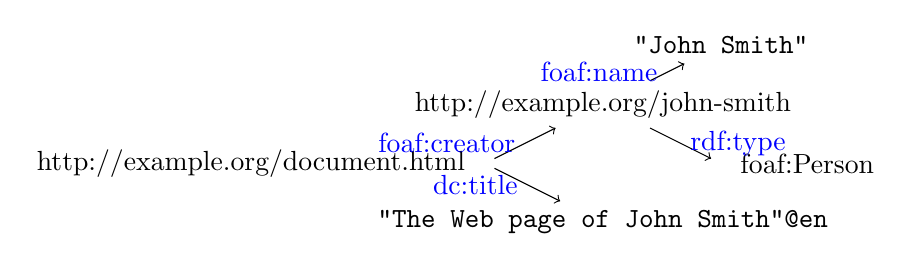
\begin{tikzpicture}[grow=right,->]
  \node[label=left:{\url{http://example.org/document.html}}] {}
    child { node {\texttt{"The Web page of John Smith"@en}}
      edge from parent
      node[left] {\textcolor{blue}{dc:title}}}
    child { node {\url{http://example.org/john-smith}}
      child { node[label=right:{foaf:Person}] {}
        edge from parent
        node[right,align=left] {\textcolor{blue}{rdf:type}}}
      child { node {\texttt{"John Smith"}}
        edge from parent
        node[left] {\textcolor{blue}{foaf:name}}}
      edge from parent
      node[left] {\textcolor{blue}{foaf:creator}};
    };
\end{tikzpicture}}}

  \caption{A graph of the \acroshort{RDF} document from Figure
    \ref{fig:rdf-doc}}
\end{figure}

%%% Linked Data
%%%   <http://www.w3.org/DesignIssues/LinkedData.html>
%%%
%%% Tim Berners-Lee: The next web
%%%   <http://www.ted.com/talks/tim_berners_lee_on_the_next_web>
%%%
%%% The SPARQL Query Language for RDF (SPARQL) and the (at the time of
%%% writing only drafted) Linked Data Fragments RDF query interfaces
%%%   <http://www.w3.org/TR/rdf-sparql-query/>
%%%   <http://linkeddatafragments.org/specification/>
%%%
%%% The Rule Interchange Format (RIF)
%%%   <http://www.w3.org/TR/rif-overview/>
        
\section{Document Preparation Systems}
Some of the existing markup is directly tied with specific \acropl{DPS}.
These \acropl{DPS} can be dichotomized into \term*{batch-oriented}%
\acroindex[!batch-oriented]{DPS}, which process marked up input
text documents into printable output documents in a page description language on
demand, and \term*{interactive}\acroindex[!interactive]{DPS}, which
allow the user to directly edit an approximation of the output document via a
visual editor. Also called \acronym{WYSIWYG}, interactive \acropl{DPS} exchange
mild learning curve for more primitive typesetting algorithms that don't stand
in the way of interactivity and for reduced flexibility stemming from the usage
of a \acronym{GUI}, which, although often intuitive for simple tasks, seldom
matches the power of the markup languages used by batch-oriented \acropl{DPS}.

\subsection{Batch-oriented Systems}
One of the archetypal batch-oriented \acropl{DPS} are \cliutil*{troff}%
\index{troff@\cliutil*{troff}}, whose function is to produce output for general
printers, and \cliutil*{nroff}%
\index{nroff@\cliutil*{nroff}|see{\cliutil*{troff}}}, whose function is to
produce output for line printers and text terminals. Both tools were developed
as a proprietary software for the Unix operating system at the beginning of
1970s by \acronym{ATnT}. An alternative to \cliutil*{nroff} and \cliutil*{troff}
is \cliutil*{groff}\index{groff@\cliutil*{groff}|see{\cliutil*{troff}}}, which
was developed as a free software in 1980 by \acronym{GNU}. \Cliutil*{groff}
combines the capabilities of both tools and is still used extensively for the
markup of documentation in \Unices, although more advanced alternatives for
general typesetting (such as \TeX) exist. The associated markup language
combines presentation markup with programming constructs and allows the
definition of logical markup in the form of user macros. Standard macro
packages, such as \identifier{man} for the
\index{troff@\cliutil*{troff}!\identifier{man}} formatting of documentation,
\identifier{me} \index{troff@\cliutil*{troff}!\identifier{me}} for the creation
of research papers, or the more recent \identifier{mom}
\index{troff@\cliutil*{troff}!\identifier{mom}} for general typesetting tasks
are typically distributed along with the system. Special markup invokes
preprocessors that can be used for the typesetting of tables, equations, and
vector graphics.

\begin{figure}
  \fbox{\includegraphics[clip,trim=1.7cm 12cm 1.7cm 1.3cm,%
    width=0.975\textwidth]{examples/02/poe-groff.pdf}}
  \inputcode[groff]{examples/02/poe.groff}
  \caption{An excerpt from the beginning of \person{Edgar Allen Poe}'s
    \work*{Cask of Amontillado}\workindex{the Cask of Amontillado} formatted
    via the \identifier{mom} macro package of \cliutil*{groff}.}
  \label{fig:poe}
\end{figure}

%%% The Groff and Friends HOWTO
%%%   <http://troff.org/TheGroffFriendsHowto.pdf>
%%%
%%% Writing Macros
%%%   <https://www.gnu.org/software/groff/manual/html_node/Writing-Macros.html>
%%%
%%% A User's Guide to the Lout Document Formatting System
%%%   <https://www.urz.uni-heidelberg.de/imperia/md/content/urz/programme/text/lout.pdf>

Another notable batch-oriented \acronym{DPS} is \TeX\index{TeX@\TeX}\footnote{
  The circumstances that led to the creation of \TeX\ and the surrounding tools
  are thoroughly documented in \citework{knuth98}.
}, which was developed and consequently released to the public domain in 1970s
by an American professor of computer science \person{Donald Knuth} after he had
received galley proofs for the second volume of his monograph, \work{the Art of
Computer Programming}, and found the appearance of mathematical formulae
distasteful. As a result, the typesetting of mathematics is a central theme in
\TeX, rather than an afterthought, which differentiates it from most other
\acropl{DPS} and which largely contributed to the massive popularity \TeX\ has
attained in academia. Much like in the case of \cliutil*{troff} and its
derivatives, the language of \TeX\ is ripe with typographic and programming
primitives and doesn't by itself contain logical markup. The language, however,
allows for the creation of user macros. An example of a macro package that makes
it possible to create documents of various classes with pure logical markup is
\LaTeX\index{LaTeX@\LaTeX}: the standard markup language for academic and
technical documents.

\begin{figure}
  \inputcode[tex]{examples/02/poe.tex}
  \caption{The document from Figure \ref{fig:poe} reformulated in \TeX\ using
    \hologo{plainTeX} macros and the primitives of \hologo{eTeX} and
    \hologo{pdfTeX}}
\end{figure}

\subsection{Interactive Systems}
Interactive \acropl{DPS} come in two distinctive flavors. Word processors
\acroindex[!interactive!word processing]{DPS} are the digital progeny of the
typewriter machine, with which they share the main function of fast text
capture. The typewriter output documents served largely as a manuscript for
designers and typographers, who then produced the actual published work. With
the advent of personal computing and the Web, self-publishing became more
approachable to the general public, and modern word processors can be used not
only to write but also to design and typeset documents, although the offered
functionally is typically constrained by user experience demands. This concern
is not shared by \term*{\acronym{DTP}
software}\acroindex[!interactive!desktop publishing]{DPS}, which provides
refined control over the resulting page layout and the typesetting primitives.
The ability to produce documents comparable to those set using traditional
typography comes at the expense of a steeper learning curve.

Most interactive \acropl{DPS} will provide a means to mark up sections of text.
Presentation markup performs direct changes of typographic properties, such as
the face, family, variant, color, or the size of the font that is used to
typeset the text. Logical markup enables the classification of sections of text
with the ability to set up the design of each class later on. This decouples
writing and markup from design and makes it easy to change the design of the
entire document and difficult to produce inconsistent design.

\begin{figure}
  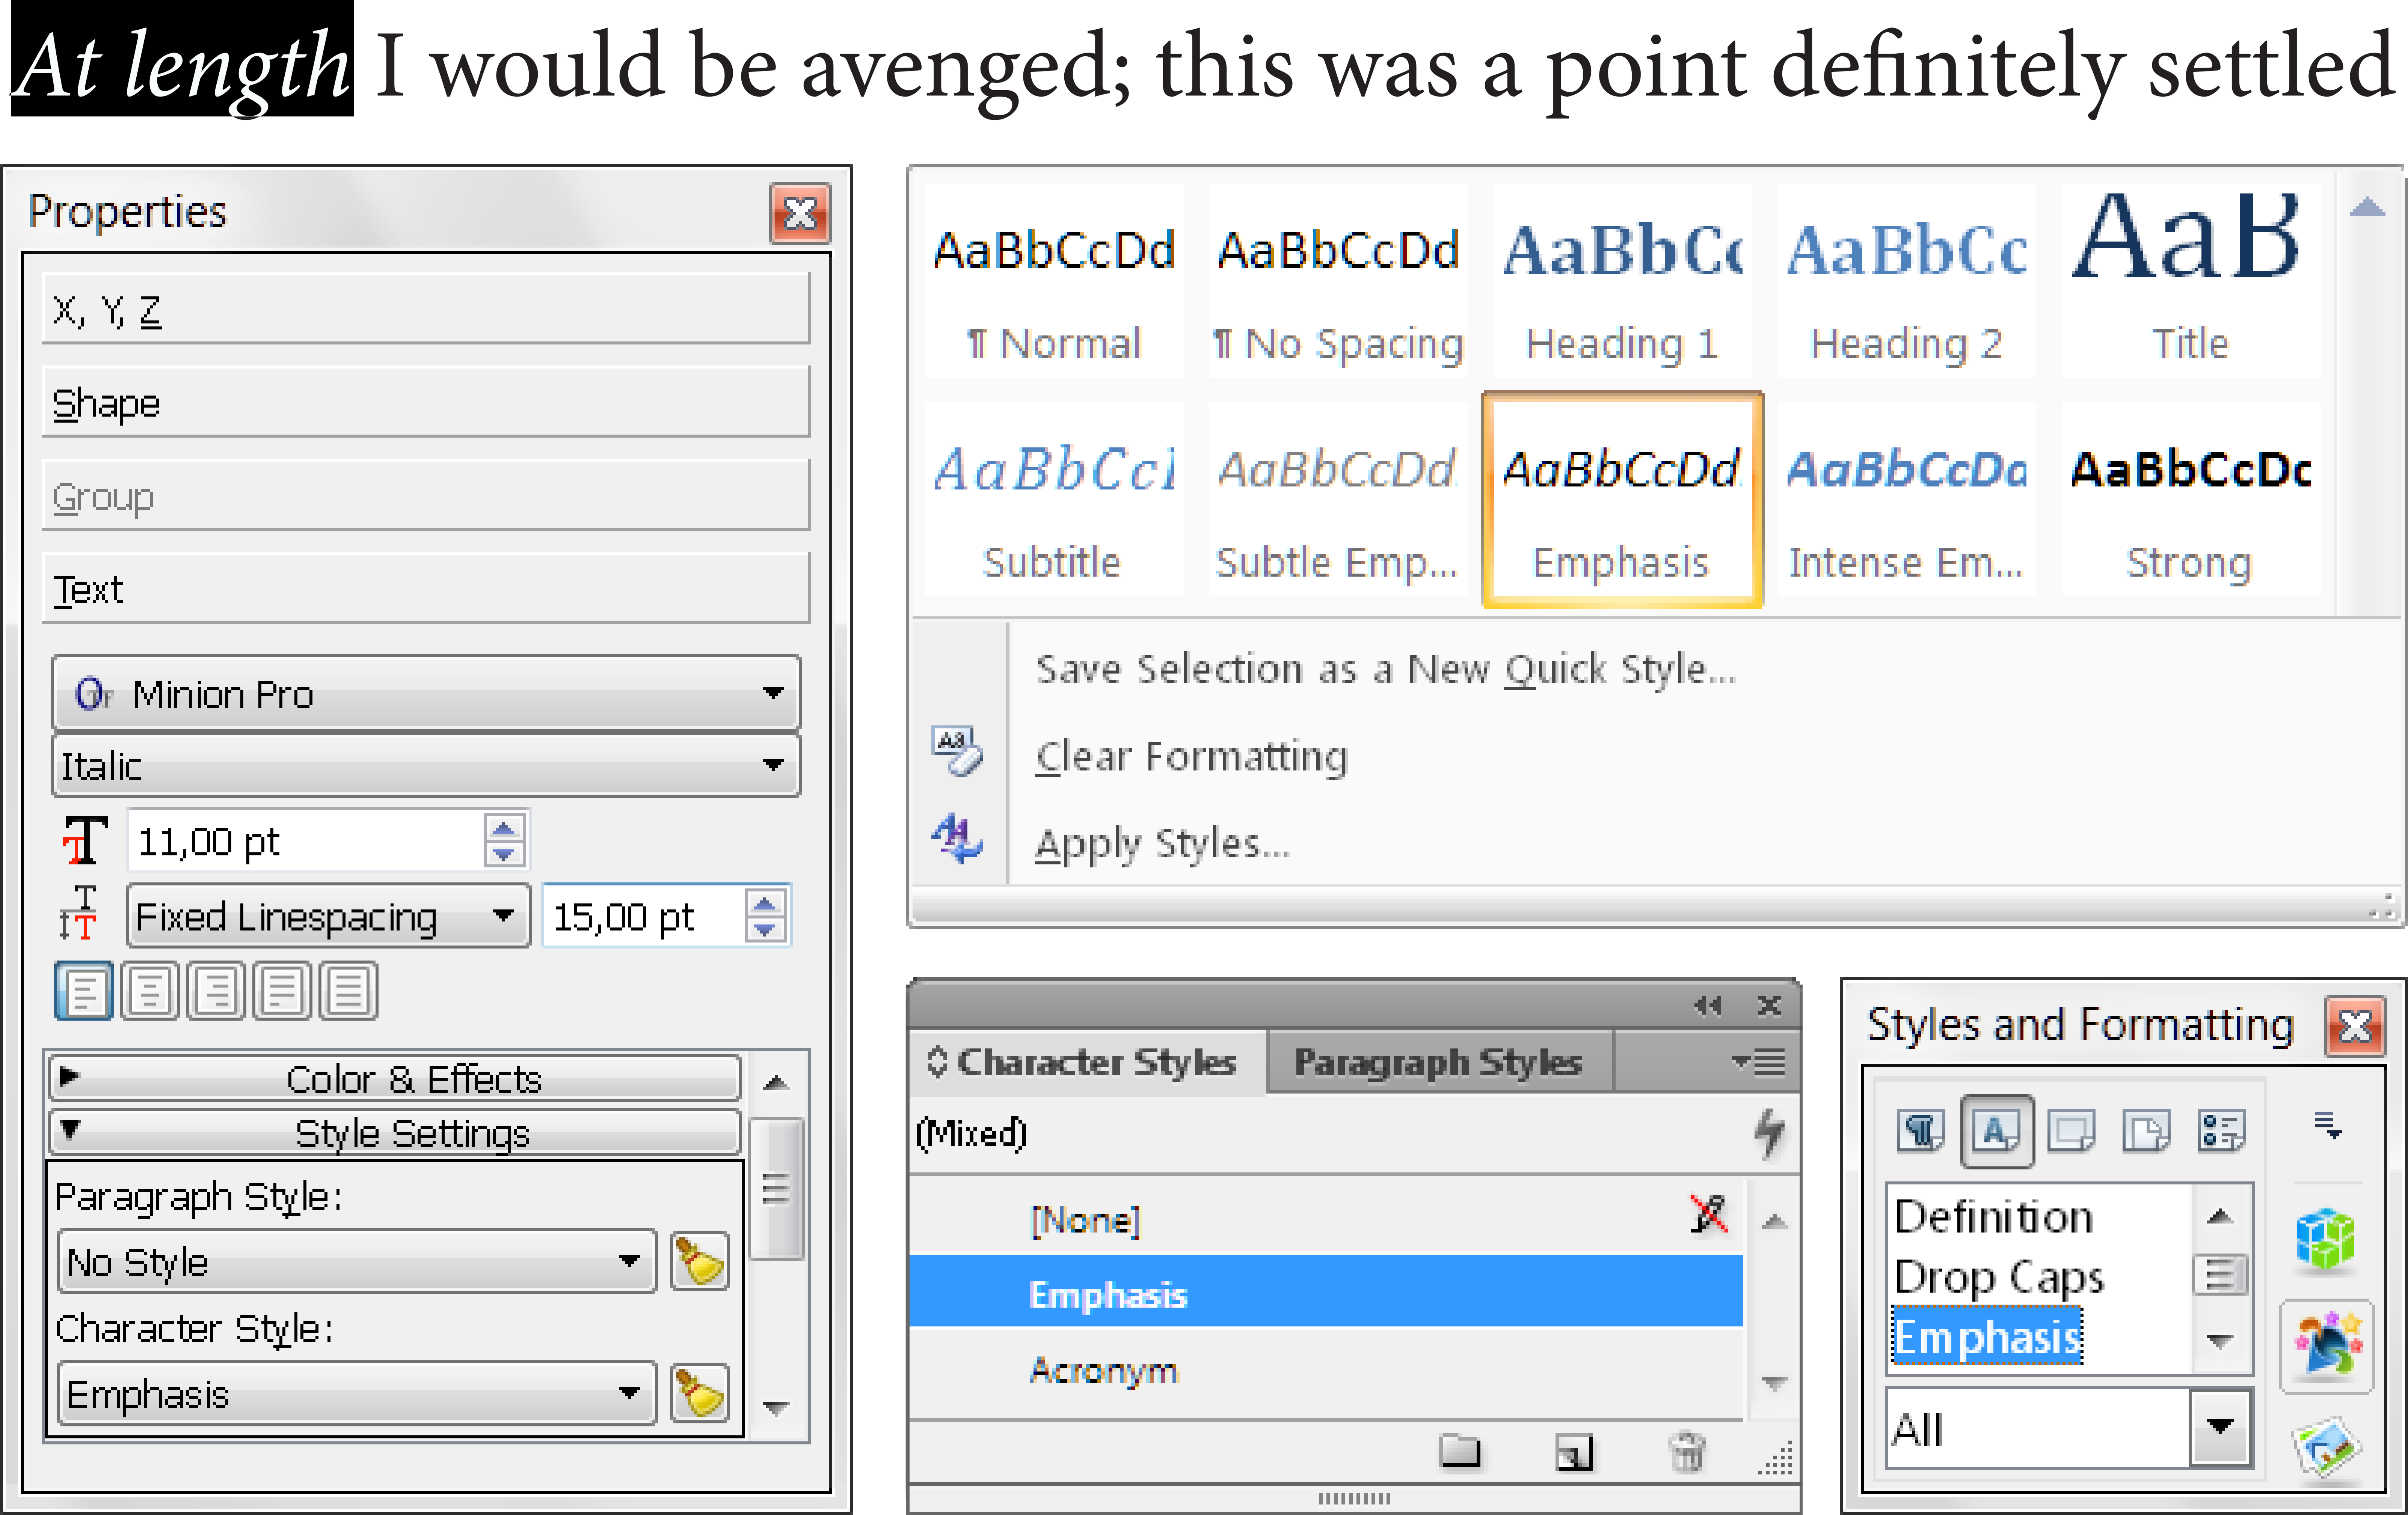
\includegraphics[width=\textwidth]{examples/02/interactive-editors.png}
  \caption{Logical markup in the interactive \acropl{DPS} of \inx{Scribus}
    (left), \inx{Microsoft Word} (top), \inx{Adobe InDesign} (bottom left) and
    \inx{Apache OpenOffice} (bottom right)}
\end{figure}

\section{Lightweight Markup Languages}
Parallel to the heavy-duty applications of \acronym{SGML} and \acronym{XML},
there runs a vein of markup languages that give priority to unobtrusiveness and
legibility over raw expressive power. Rooted in the reality of computer text
terminals with limited formatting capabilities, \termpl{lightweight markup
language} leverage punctuation and indentation to produce comparatively weak and
domain-specific, but also humane, highly intuitive, and often profoundly
beautiful markup that is easy to both read and write. Examples of lightweight
markup languages include \inx{Markdown}, \inx{Creole}, \inx{AsciiDoc},
\inx{MakeDoc}, \inx{Setext}, or \inx{Wikicode}.  Lightweight markup languages
are typically supplemented by tools that enable the conversion to more general
markup languages, such as \acronym{HTML}. Also typical is the existence of
numerous flavors of every lightweight markup language, which represent its
different use cases.
